\chapter{Abstract Finite State Model of inherent noise}
\label{cha:bgp_fsm}

\fxfatal{explicit that the fsms are produced by the experiments with the des}

The incremental nature of \ac{BGP} suggests that is possible to study the
evolution of the protocol looking to the events that have been triggered
and the causes of them.
A model that can give this sort of information would be helpful to debug
the protocol, analyze faulty situations or prevent them.
The main idea behind this model of the protocol has been taken and
expanded from~\cite{griffinFSM}.
I'm going to show that inferring information from \ac{BGP} events and actions
is more difficult than expected.
In fact, due to the \textit{Path Exploration} problem
nodes will experience an explosion in the number of possible evolutions,
presented in \Cref{sec:bgp_fsm_explosion}.
In addition to that, multiple inputs can lead to the same output of the node,
for this reason, it is not enough to know it to infer a precise input signal,
showed in \Cref{sec:bgp_fsm_experiments}.
Furthermore, \ac{MRAI} can make the situation even more complicated, increasing
the number of transitions because of all the new possible combinations of
inputs.

\section{BGP generalization}
\label{sec:bgp_generalization}

The main idea behind the \ac{BGP} \ac{FSM} is to represent the knowledge as
states and a set of messages as transitions.
The knowledge is represented by the actual routes that the node knows on how
to reach a single destination, we will have a different \ac{FSM} for every
destination.
Transitions encode the messages that a node has received to trigger the state change,
on the edges are also inserted the response messages that the node will transmit.
We can see an example of these transitions in \Cref{fig:fsm_example}

\begin{figure}[h]
    \begin{center}
        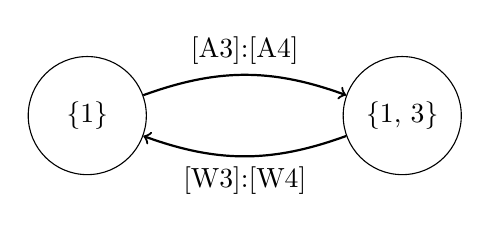
\begin{tikzpicture}[scale=0.2, state/.style={draw=black,circle,inner sep=0pt}]
	\node [state, minimum size=1.5cm] (s1) at (0,0) {\{1\}}; 
	\node [state, minimum size=1.5cm] (s2) at (20,0) {\{1, 3\}};
	%\draw[arrow](B1.west) to [out=190,in=170] node[above]{Flow: $\alpha$ } (S1.west);
	\draw [thick, ->] (s1) to[out=20, in=160] node[above]{[\q{A3}]:[\q{A4}]} (s2); 
	\draw [thick, ->] (s2) to[out=-160, in=-20] node[below]{[\q{W3}]:[\q{W4}]} (s1);
\end{tikzpicture}                        

    \end{center}
	\caption{Example of the \ac{BGP} \ac{FSM} state transition}
    \label{fig:fsm_example}
\end{figure}

In \Cref{fig:fsm_example} there are two states, both represent the knowledge of
the node, the first one represents the \ac{RIB} with just the route \num{1}, in
the second state the \ac{RIB} will contain both the routes \num{1} and \num{3}.
This transition is caused by the reception of the advertisement of the route
\num{3} and will cause the transmission of another advertisement.
The opposite transition is caused by the reception of the withdraw of the route
\num{3} with the consequent withdraw of the route \num{4}.
The route which id is bold represent the actual best path chosen by the node, in
this case the reception of \q{A3} provoke the change of the best path, noticeable
in the second state where the route \num{3} is bold.

Thanks to \ac{MRAI} the evaluation of multiple messages could be delayed and
provoke then the compression of them.
For this reason on the edges is possible to see multiple messages, for example
\q{[A1W1A1]}, that will be compressed in \q{[A1]} and then evaluated.
The output part of the transition will be influenced by \ac{MRAI}, the output
message strongly depend on the number of messages that the node was able
to compressed.

%\begin{itemize}
%    \item BGP as an FSM main idea
%    \item signalling transmutation
%\end{itemize}

\section{BGP FSM experiments}
\label{sec:bgp_fsm_experiments}

The first experiments that I executed are about the translation of a single
node evolution in a \ac{FSM}.
The goal is to reproduce what has been shown in~\cite{griffinFSM}.
The graph used for the study is presented in \cref{fig:griffin_fig_4}.

\begin{figure}[h]
    \begin{center}
        \begin{tikzpicture}[scale=0.2, every node/.style={draw=black,circle,inner sep=0pt}]
    \node [minimum size=1cm] (1) at (0,0) {1}; 
    \node [minimum size=1cm] (2) at (-8,-8) {2}; 
    \node [minimum size=1cm] (3) at (8,-8) {3}; 
    \node [minimum size=1cm] (4) at (0,-16) {4}; 
    \node [minimum size=1cm] (5) at (0,-24) {5}; 
	\draw [thick, ->] (0, 5) -- (1);
    \draw [thick, ->] (1) -- (2);
    \draw [thick, ->] (1) -- (3);
    \draw [thick, ->] (2) -- (4);
    \draw [thick, ->] (3) -- (4);
    \draw [thick, ->] (3) -- (5);
    \draw [thick, ->] (4) -- (5);
	\draw [thick, ->] (5) -- (0, -30)
\end{tikzpicture}                                                       


    \end{center}
	\caption{Graph from fig 4 of~\cite{griffinFSM} used to study the \ac{FSM}
		of the nodes}
    \label{fig:griffin_fig_4}
\end{figure}

This topology, \Cref{fig:griffin_fig_4}, present a \ac{SPP} with five node~\cite{griffin2002stable}.
The \ac{SPP} model is used to eliminate much of the complexity of \ac{BGP}.
The arrows in the graph represent the flow of information, node \num{1} is the one
that will receive a new route to reach a hypothetical destination and it will
spread this information using an \ac{ADV} towards all its neighbours.
After a while node \num{1} will also distribute the withdraw of that route.
The translation to the \ac{CFSM} will use an enumeration to encode all the
paths that a single node will encounter, for example, the path \q{5 3 1} will
be converted in \textit{a3}, each path has its own identifier.
In case of withdrawing the route will be encoded as \textit{w3}.

The properties of the environment for this experiment are listed in \Cref{tbl:fig_4_example}.

\begin{table}[h]
	\begin{center}
	\begin{tabular}{ || m{4cm}| m{8cm} || } 
	\hline
	Property & Value \\ 
	\hline \hline
	Seeds & $[1, 50]$ \\ 
	\hline
	Signaling & \q{AW} \\
	\hline
	Withdraws delay & Uniform distribution between \SI{20}{\second} and \SI{30}{\second} \\ 
	\hline
	Announcement delay & Uniform distribution between \SI{20}{\second} and \SI{30}{\second} \\ 
	\hline
	MRAI & \SI{0}{\second} for every link \\
	\hline
	Link delay & Uniform distribution between \SI{0.001}{\second} adn \SI{1}{\second}, uniform distribution between \SI{0.012}{\second} and \SI{3}{\second} \\
	\hline
	\end{tabular}
\end{center}

	\caption{FSM example environment properties}
	\label{tbl:fig_4_example}
\end{table}

The total number of runs generated by this environment is \num{100} (\num{50} seeds
and \num{2} possible delay distributions).
\ac{MRAI} has been setted to \SI{0}{\second} in order to be ininfluent
during the simulation.

The two nodes we are most interested are node \num{4} and node \num{5}, because of their
position after a fork.
The first one is going to receive the messages of node \num{2} and \num{3}, for
sure there will be two announcements and two withdraws because of the signal
imposed on node 1.
Node \num{2} will share an announcement followed by a withdraw and the same node
\num{3}.
Those messages can be reordered in different way, always respecting the local
order.
For each sequence the node \num{4} can take different decision, for
example use the path though node \num{3} and then change its decision using the
one received from node \num{2}.
Is possible to see all the possible combinations of inputs and outputs of node
\num{4} in \Cref{tbl:fig_4_node4_possible_inputs}.
The messages from node \num{2} and \num{3} would have a single unique id, because
both the nodes only know one path to the destination.
While, node \num{4} has the possibility to propagate two different paths, each
one with a unique id.
The output signals of node \num{4} would be part of the set of all the possible
inputs of node \num{5}.

\begin{table}[h]
	\begin{center}
	\begin{tabular}{ || m{3cm}| m{3cm} || }
	\hline
	Input signal & Output signal\\
	\hline \hline
	$a2a3w2w3$ & $a4a5w4$ \\
	$a2a3w3w2$ & $a4w4$ \\
	$a3a2w2w3$ & $a5a4a5w5$ \\
	$a3a2w3w2$ & $a5a4w4$ \\
	$a2w2a3w3$ & $a4w4a5w5$ \\
	$a3w3a2w2$ & $a5w5a4w4$ \\
	\hline
	\end{tabular}
\end{center}


	\caption{Node 4 different possible inputs and output}
	\label{tbl:fig_4_node4_possible_inputs}
\end{table}

The node \num{5} is going to receive all the possible outputs from node \num{3} and
\num{4}.
The number of input signals of node \num{5} is composed by all the possible
combinations of messages in the output set of node \num{4} and \num{3}.
The total number of possible inputs for node \num{4} is \num{6}, like
showed in \Cref{tbl:fig_4_node4_possible_inputs}, for node \num{5} is going
to be \num{71}.
In \Cref{tbl:fig_4_node4_possible_inputs} is possible to notice that
there are no inputs that produce the same output, thats not true also for
the node \num{5}.
In fact, node \num{5} has in total \num{52} unique possible output sequence,
given by all the \num{71} different inputs.

From the \num{100} total runs, we can generate the \ac{CFSM} of node \num{4} and
node \num{5}, in order to be able to study how the nodes react to different
input signals.
The two \ac{CFSM} are presented in \Cref{fig:fsm_griffin_fig4}.

\begin{figure}[h]
     \centering
     \begin{subfigure}[b]{0.49\textwidth}
         \centering
         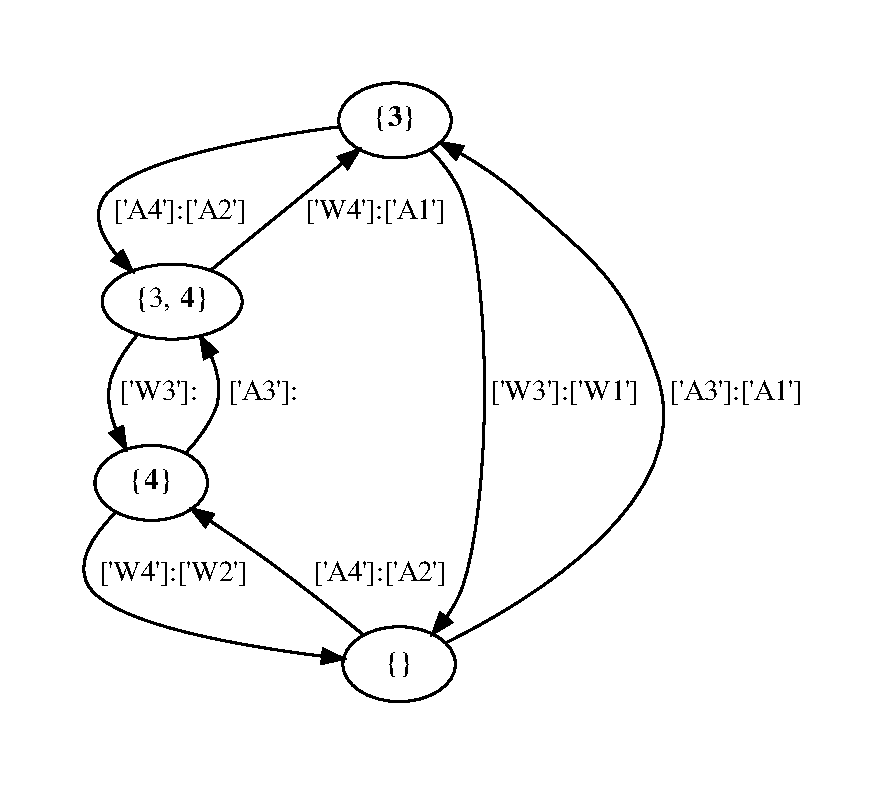
\includegraphics[width=\textwidth]{images/fsm/fig_4_4.pdf}
		 \caption{Node \num{4} \ac{CFSM} from the environment of \Cref{tbl:fig_4_example}}
         \label{fig:fsm_node4}
     \end{subfigure}
     \hfill
     \begin{subfigure}[b]{0.49\textwidth}
         \centering
         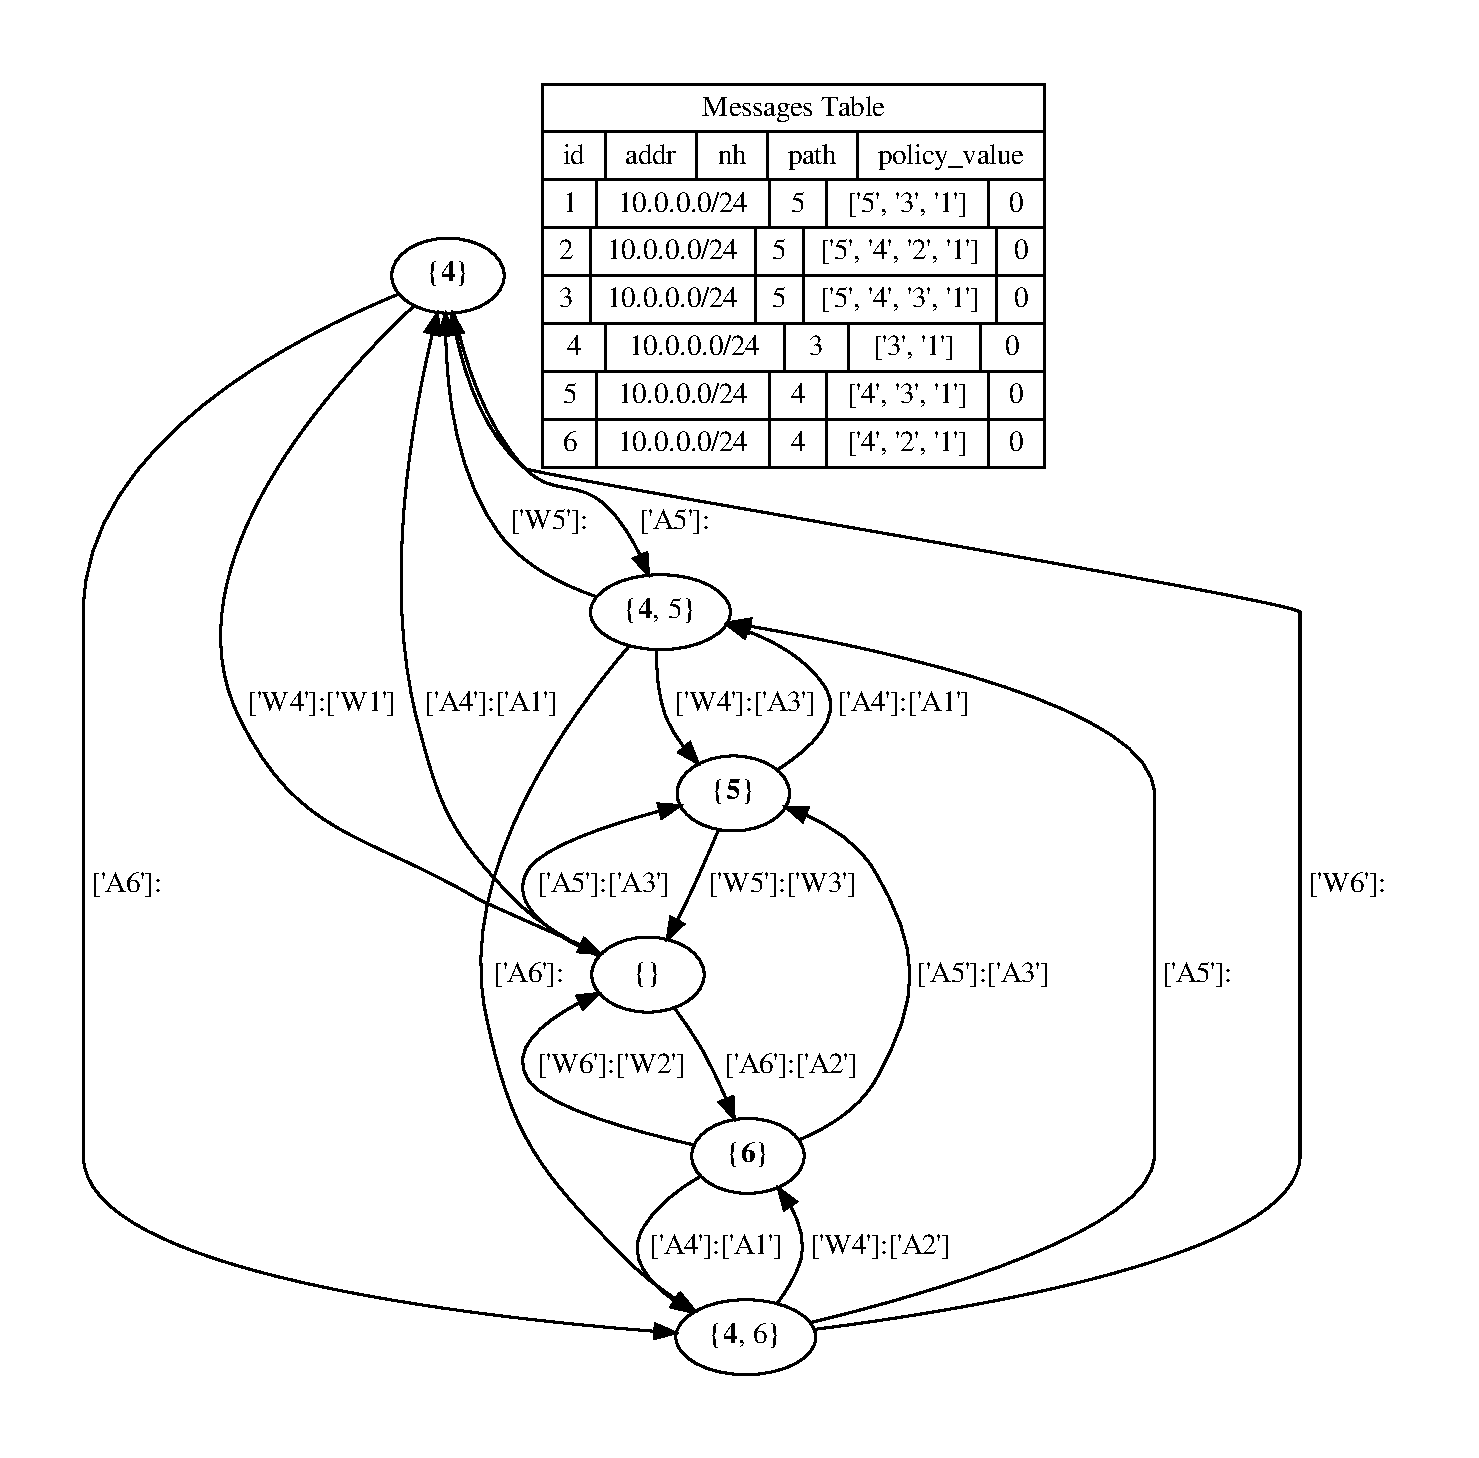
\includegraphics[width=\textwidth]{images/fsm/fig_4_5.pdf}
		 \caption{Node \num{5} \ac{CFSM} from the environment of \Cref{tbl:fig_4_example}}
         \label{fig:fsm_node5}
     \end{subfigure}
		\caption{\ac{CFSM} of nodes \num{4} and \num{5} of the graph
			\Cref{fig:griffin_fig_4} with an input signal of \q{AW},
			\num{100} total different runs, \ac{MRAI} ininfluent.
			\fxfatal{Remove message tables?}}
        \label{fig:fsm_griffin_fig4}
\end{figure}

The states of the \ac{CFSM} in \Cref{fig:fsm_griffin_fig4} are represented by the
knowledge of the nodes, composed by the routes that are in the \ac{RIB} of the node.
The bold value is the actual best route to the destination chosen by the node.
If in the state transition to a new state the best path is not affected then the
node will not transmit the new route to its neighbours, for an example take
a look to \Cref{fig:fsm_node4} from the state $\{4\}$ to the state $\{3, 4\}$
where the node \num{4} will learn a new route that is not the best one.

The effects of the implicit withdraw can be seen in \Cref{fig:fsm_node5}
the transition from $\{4, 6\}$ to $\{4, 5\}$ thanks to the reception of the
announcement $a5$ from the node \num{4}.

As written in~\cite{griffinFSM}, I would like to underline the fact that, given
the \num{52} unique possible outputs of the node \num{5} it would be very difficult
to infer the initial signal that provokes all the transitions.

We can also analyze those output signals, knowing all the events for each single
run we can infer which were the most common output signals experienced by a single node.
Is sufficient to take all the transmitted messages of a node and look the sequence
of advertisement and withdraws.

\begin{figure}[h]
     \centering
     \begin{subfigure}[b]{0.49\textwidth}
         \centering
         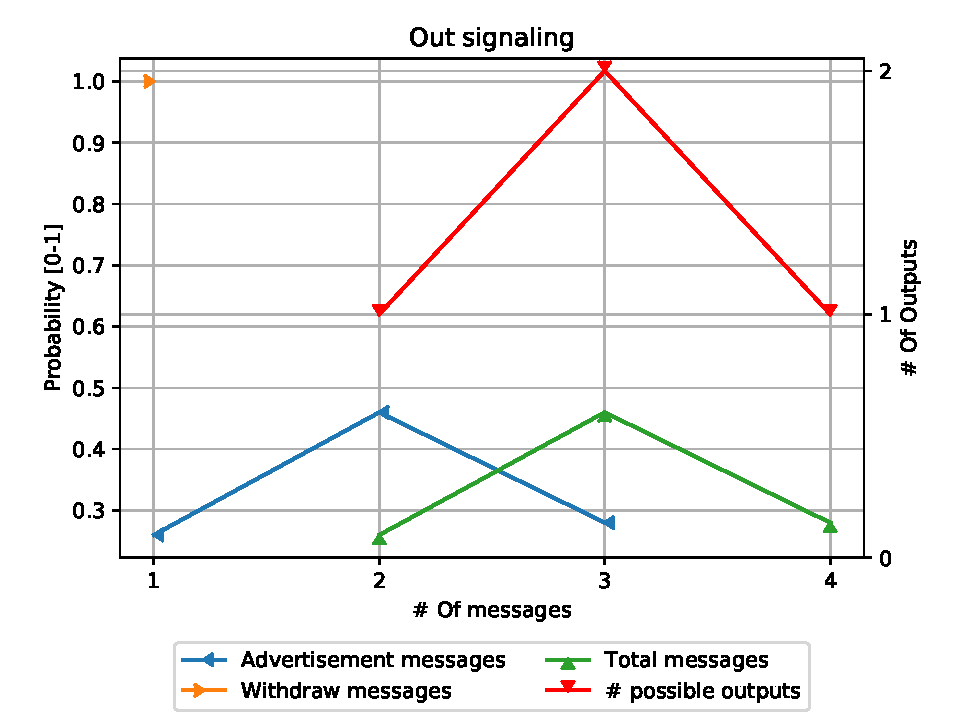
\includegraphics[width=\textwidth]{images/signal_study/fig_4/fig_4_4_signaling_nmessage_prob.pdf}
		 \caption{Node \num{4} output signals study}
         \label{fig:signal_node4}
     \end{subfigure}
     \hfill
     \begin{subfigure}[b]{0.49\textwidth}
         \centering
         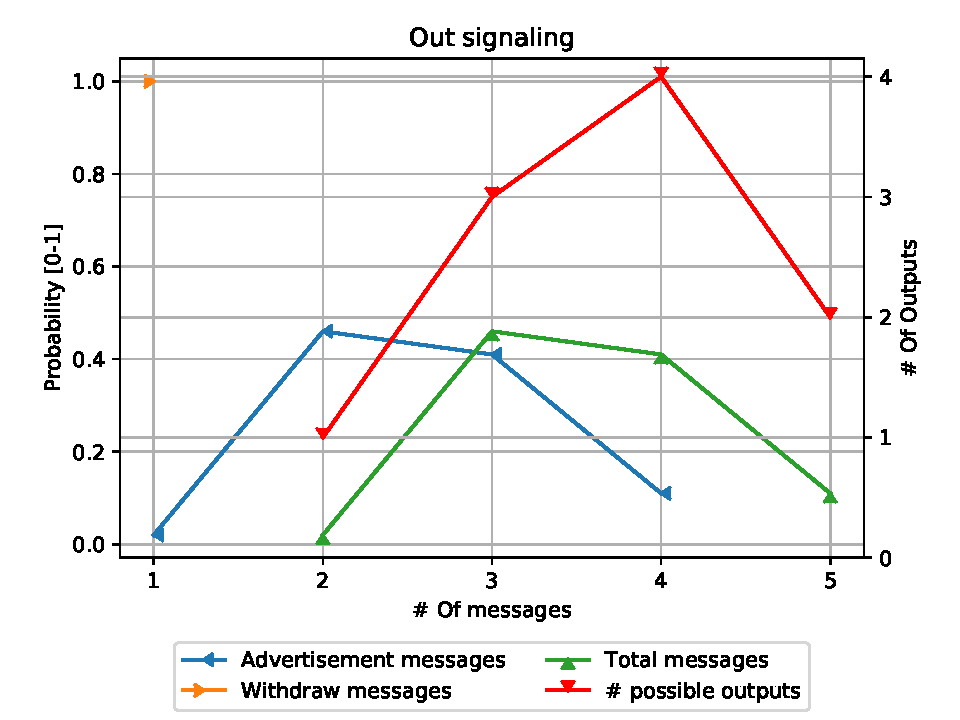
\includegraphics[width=\textwidth]{images/signal_study/fig_4/fig_4_5_signaling_nmessage_prob.pdf}
		 \caption{Node \num{5} output signals study}
         \label{fig:signal_node5}
     \end{subfigure}
		\caption{Output signal study of nodes \num{4} and \num{5} of the graph
			\Cref{fig:griffin_fig_4} with an input signal of \q{AW} at node \num{1},
			\num{100} of total runs, \ac{MRAI} ininfluent}
        \label{fig:signal_griffin_fig4}
\end{figure}

The plots in \Cref{fig:signal_griffin_fig4} represents the probability of an
output signal of a certain length to be detected and the number of unique output signals
that have been found for each possible length.
The $x$ axis represents the number of messages in the output signal, a message
is a single announcement or withdraw.
The first $y$ axis represents the probability to see a certain number of messages
taking a random output signal from the set.
Three lines refers to this axis, the blue one represents the
number of advertisement messages in the output signal correlated with the
respective probability.
For example, in \Cref{fig:signal_node4} there is a probability around $0.45$ to have
exactly two advertisement messages per output signal. And respectively a probability
slightly larger than $0.25$ to have only one advertisement or three.
We can also notice that we didn't see more than three advertisements or less than one.
The green line instead represents the total number of messages in the signal,
without distinguishing between advertisement and withdraws.
By the fact that we will always experience one withdraw (the orange line) the
green line is simply shifted by one unit in respect of the advertisement line.
There is a probability around the $0.45$ to have exactly \num{3} messages in the
output signal.
The second $y$ axis refers to the number of unique output signals encountered and
their length.
For example, in \Cref{fig:signal_node5} we will have \num{1} unique output signal
of length \num{2}, \num{3} signals of length \num{3}, \num{4} of length \num{4}
and \num{2} of length \num{5}.
In total we saw \num{10} different unique signals on \num{100} different runs.

Those plots do not give a complete perspective of all the possible outputs
that can be generated but only the one encountered during the runs.
In fact, during the \num{100} runs, we encountered only the output signals listed
in \cref{tbl:signals}.

\begin{table}[h]
	\begin{subtable}[h]{0.45\textwidth}
		\begin{center}
	\begin{tabular}{ || m{3cm}| m{3cm} || } 
	\hline
	Signal & Frequency\\ 
	\hline \hline
		$a1a2a1w1$ & \num{28} \\
		$a2a1w1$ & \num{23} \\
		$a2w2$ & \num{26} \\
		$a1a2w2$ & \num{23} \\
	\hline
	\end{tabular}
\end{center}


		\caption{Node \num{4} output signals encountered}
		\label{tab:node4_outSignals}
    \end{subtable}
	\hfill
	\begin{subtable}[h]{0.45\textwidth}
		\begin{center}
	\begin{tabular}{ || m{3cm}| m{3cm} || } 
	\hline
	Signal & Frequency\\ 
	\hline \hline
	$a1a2a3w3$ & \num{15}\\
	$a1a3w3$ & \num{16}\\
	$a2a1a2w2$ & \num{19}\\
	$a1a2w2$ & \num{28}\\
	$a1w1$ & \num{2}\\
	$a2a1a3w3$ & \num{6}\\
	$a2a1a2a3w3$ & \num{8}\\
	$a3a1a2a3w3$ & \num{3}\\
	$a2a1w1$ & \num{2}\\
	$a3a1a3w3$ & \num{1}\\
	\hline
	\end{tabular}
\end{center}


		\caption{Node \num{5} output signals encountered}
		\label{tab:node5_outSignals}
    \end{subtable}
		\caption{Node 4 and 5 different output signals encountered during the \num{100}
		runs, using the environment in \Cref{tbl:fig_4_example},
		\ac{MRAI} is ininfluent during the simulations, the signal used \q{AW}}
	\label{tbl:signals}
\end{table}


\subsection{MRAI and BGP FSM}
\label{subsec:mrai_vs_bgpfsm}

How would \ac{MRAI} affect the study of the signals produced by \Cref{fig:griffin_fig_4}?
The answer is that the number of states will be the same but the number of possible
transitions will explode because there will be a lot more possible
input signals that will be compressed and evaluated by the nodes.
Multiple transitions between the same nodes can exists because multiple input
messages could be compressed in the same set by \ac{MRAI}.
For example the sequence \q{A} could produce the same effects of the sequence
\q{AWA} once its compressed.

We can see the effects of \ac{MRAI} on the \ac{CFSM}s in \Cref{fig:fsm_griffin_fig4_MRAI}.

\begin{figure}[h]
     \centering
     \begin{subfigure}[b]{0.7\textwidth}
         \centering
         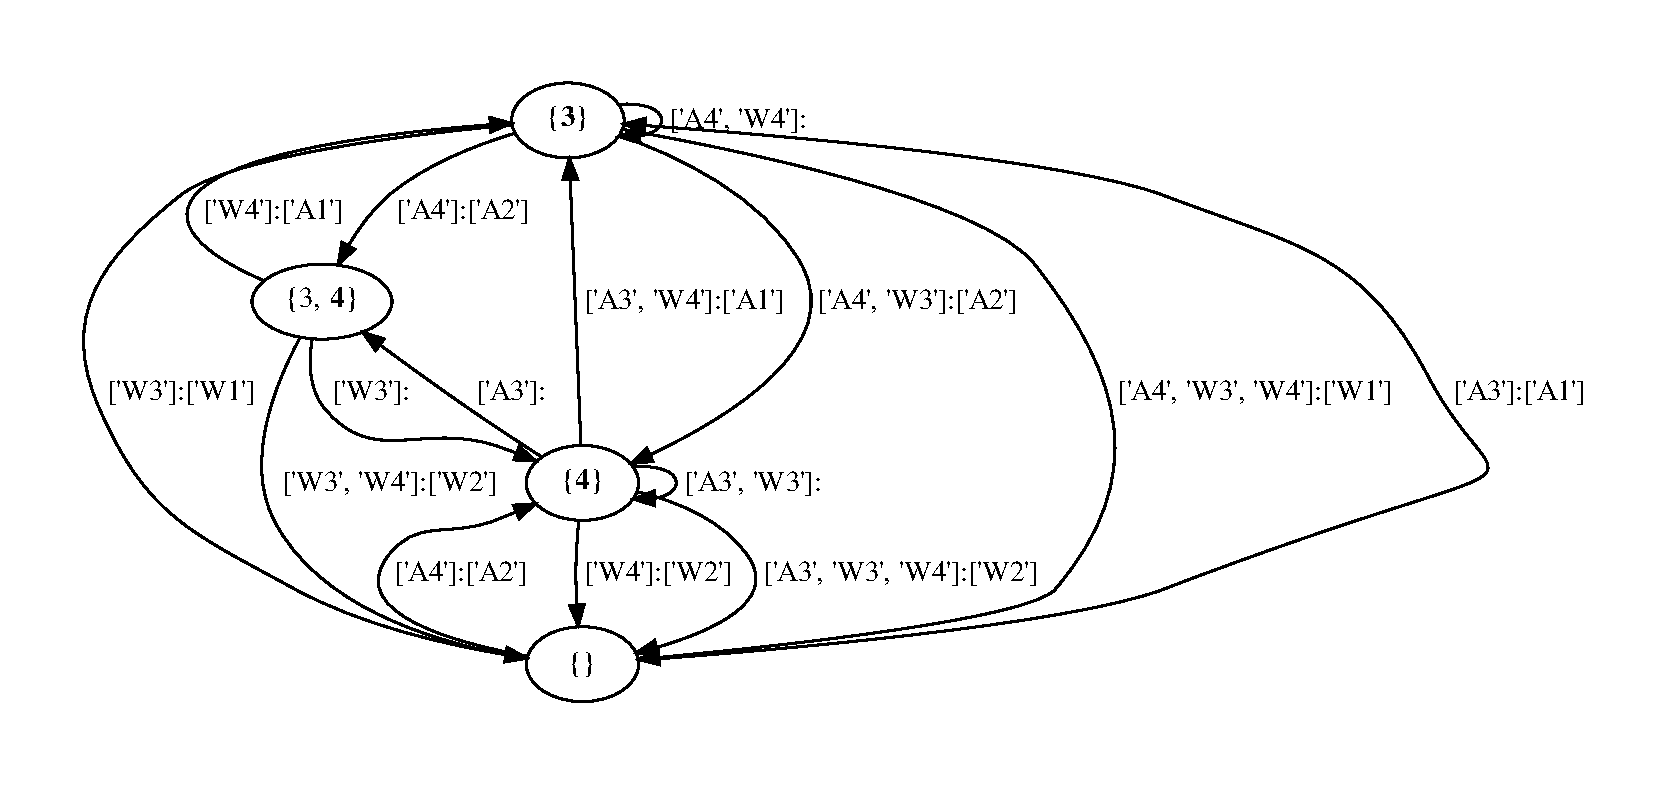
\includegraphics[width=\textwidth]{images/fsm/fig_4_4_MRAI30.pdf}
		 \caption{Node \num{4} \ac{CFSM} from the environment of \Cref{tbl:fig_4_example} with \ac{MRAI}=\SI{30}{\second}}
         \label{fig:fsm_node4_MRAI}
     \end{subfigure}
     \hfill
     \begin{subfigure}[b]{0.9\textwidth}
         \centering
         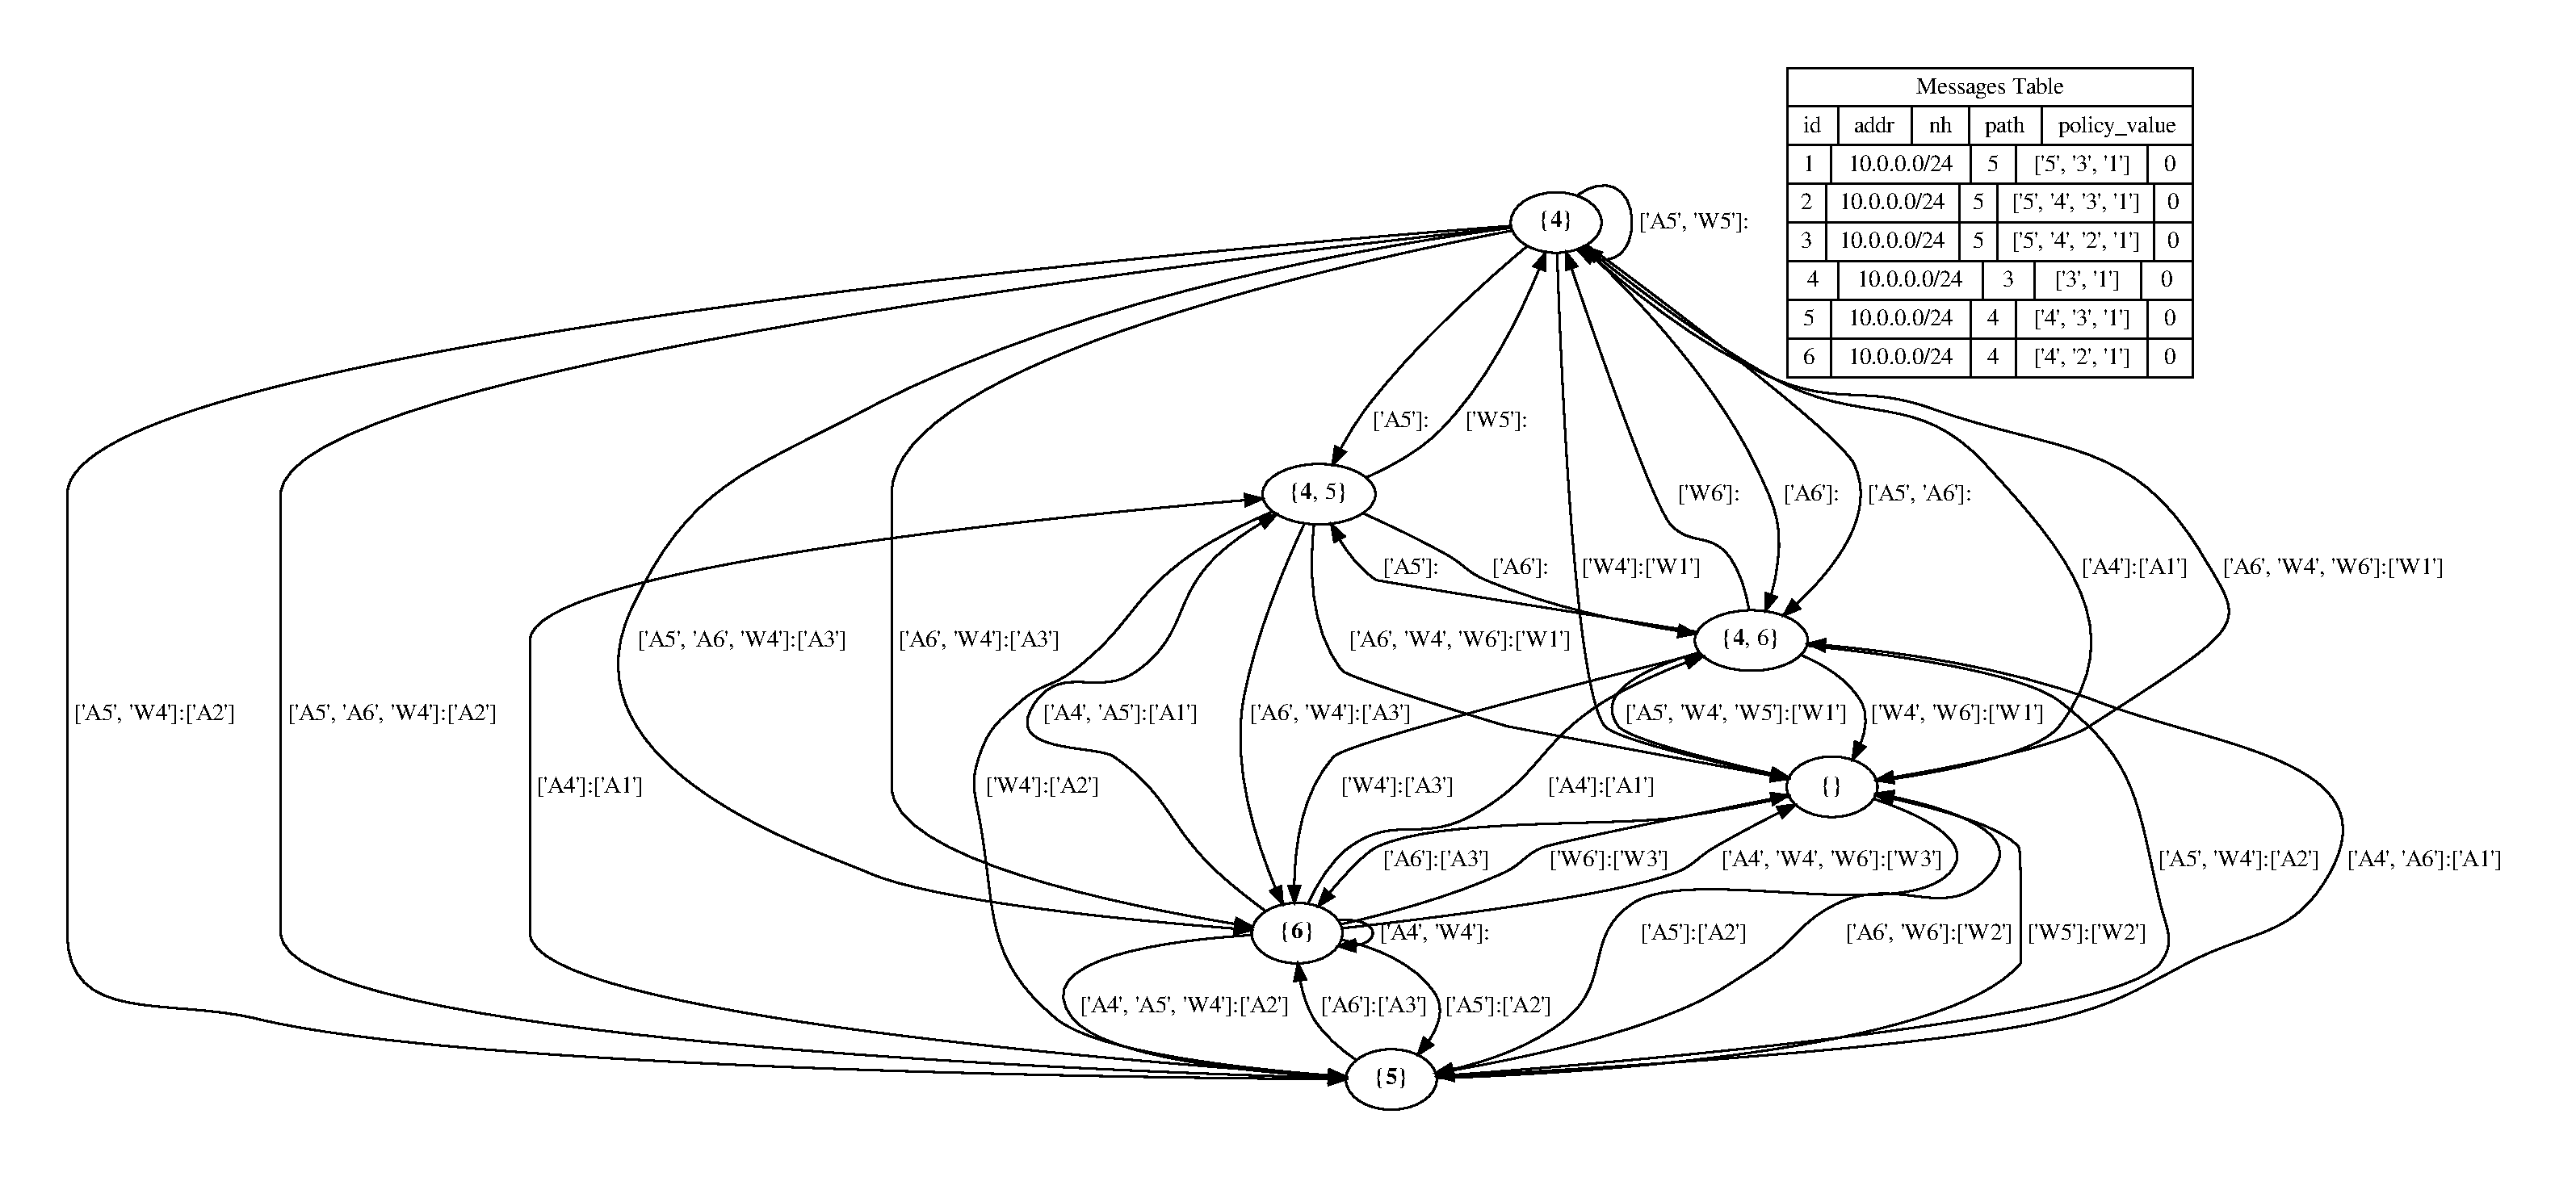
\includegraphics[width=\textwidth]{images/fsm/fig_4_5_MRAI30.pdf}
		 \caption{Node \num{5} \ac{CFSM} from the environment of \Cref{tbl:fig_4_example} with \ac{MRAI}=\SI{30}{\second}}
         \label{fig:fsm_node5_MRAI}
     \end{subfigure}
		\caption{\ac{CFSM} of nodes \num{4} and \num{5} of the graph in
			\Cref{fig:griffin_fig_4} with an input signal of \q{AW} and with
			\ac{MRAI}=\SI{30}{\second}, in total has been executed \num{100} runs}
        \label{fig:fsm_griffin_fig4_MRAI}
\end{figure}

The results in \Cref{fig:fsm_griffin_fig4_MRAI} have been generated with the same
environment of the one in \Cref{fig:fsm_griffin_fig4} but with an \ac{MRAI} value
equal to \SI{30}{\second} in each link, as defined by the \ac{RFC} \num{4271}~\cite{rfc4271}.
\Cref{fig:fsm_node4} and \Cref{fig:fsm_node4_MRAI} permits us to compare the two
\ac{CFSM}s of node \num{4}, is possible to notice a big difference in terms of edges
between one figure and the other, the first one has \num{8} transitions, the
second one \num{15}.
For the node \num{5}, we pass from \num{16} transitions in \Cref{fig:fsm_node5}
to \num{36} thanks to \ac{MRAI} in \Cref{fig:fsm_node5_MRAI}.

But the positive effects of \ac{MRAI} can be found in the output signals,
showed in \Cref{fig:signal_griffin_fig4_MRAI}.

\begin{figure}[h]
     \centering
     \begin{subfigure}[b]{0.49\textwidth}
         \centering
         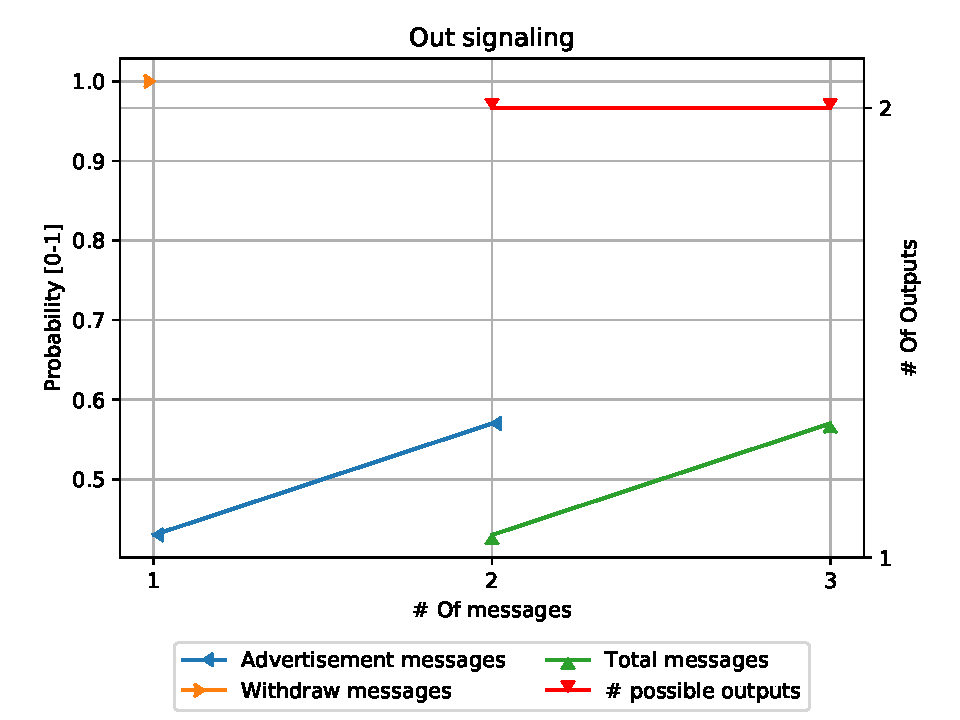
\includegraphics[width=\textwidth]{images/signal_study/fig_4_MRAI/fig_4_4_signaling_nmessage_prob.pdf}
		 \caption{Node \num{4} output signals study with \ac{MRAI}=\SI{30}{\second}}
         \label{fig:signal_node4_MRAI}
     \end{subfigure}
     \hfill
     \begin{subfigure}[b]{0.49\textwidth}
         \centering
         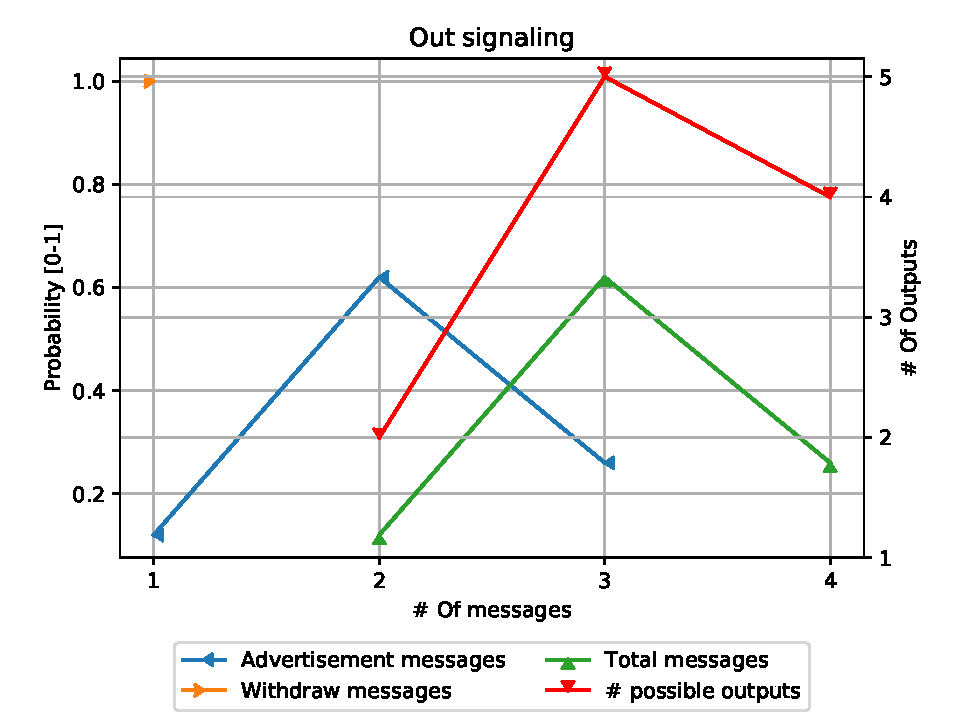
\includegraphics[width=\textwidth]{images/signal_study/fig_4_MRAI/fig_4_5_signaling_nmessage_prob.pdf}
		 \caption{Node \num{5} output signals study with \ac{MRAI}=\SI{30}{\second}}
         \label{fig:signal_node5_MRAI}
     \end{subfigure}
		\caption{Output signal study of nodes \num{4} and \num{5} of the graph
			\Cref{fig:griffin_fig_4} with an input signal of \q{AW} at node \num{1}
			with \ac{MRAI}=\SI{30}{\second} for every link}
        \label{fig:signal_griffin_fig4_MRAI}
\end{figure}

Comparing \Cref{fig:signal_node5_MRAI,fig:signal_node5} is possible to notice
that there is a different distribution in the output signals.
The $x$ axis never reaches the value of \num{5}, this means that the output signals
of the node \num{5} never used more than \num{4} messages.
While, without \ac{MRAI} there were \num{2} unique output states with \num{5}
messages, with a total frequency of \num{11}.
And we can also notice that the majority of the signals this time have a length
of \num{3} messages, instead of the previous \num{4}.
This is a hint that \ac{MRAI} can have positive effects on the number of output messages
produced by single nodes, having, however, more possible transitions to consider.

This makes inferring the input signal even more difficult because we have a lower
number of output state with a broader number of possible transitions.

\section{BGP FSM explosion}
\label{sec:bgp_fsm_explosion}

We know that \ac{MRAI} is not an easy parameter, the incorrect setting of
it can lead to an explosion of messages and an exponential convergence time.
This problem has been studied by Fabrikant et al.~\cite{fabrikant2011there} and
the origin of it has been attributed to the \textit{path exploration} issue.
This is a well-known problem in the \ac{BGP} community and it is experienced
by a node when it enters in a transitory phase where it accepts and publishes not
optimal paths towards the destination before reaching a stable state.
\textit{Path exploration} can lead to an enormous amount of messages even with
a small set of nodes~\cite{deshpande2004impact}.

As we saw in \Cref{subsec:mrai_vs_bgpfsm}, \ac{MRAI} can influence the
\ac{CFSM}s of the nodes and their output signals, which impact could it have
if it is not set correctly?

I have then created an environment that resembles the study conducted in~\cite{fabrikant2011there}
using a topology like the one described in \Cref{subsec:fabrikant_env}
with \num{3} rings and I compared different \ac{MRAI} settings.
The environment properties are presented in \Cref{tbl:fabrikant_environment}.

\begin{table}[h]
	\begin{center}
	\begin{tabular}{ || m{4cm}| m{7.5cm} || }
	\hline
	Property & Value \\
	\hline \hline
	Seeds & $[1, 30]$ \\
	\hline
		Signaling & \q{A}, \q{AW}, \q{AWA}, \q{AWAW} \\
	\hline
		Withdraws delay & Uniform distribution between \SI{5}{\second} and \SI{10}{\second}, Uniform distribution between \SI{10}{\second} and \SI{15}{\second} \\
	\hline
	Announcement delay & Uniform distribution between \SI{5}{\second} and \SI{10}{\second}, Uniform distribution between \SI{10}{\second} and \SI{15}{\second} \\
	\hline
	Link delay & Uniform distribution between \SI{0.5}{\second} adn \SI{3}{\second}, uniform distribution between \SI{2}{\second} and \SI{4}{\second} \\
	\hline
	\end{tabular}
\end{center}

	\caption{Fabrikant experiments environment}
	\label{tbl:fabrikant_environment}
\end{table}

In total, for each signalling experiment this environment produces \num{240} runs.
I have then introduced \num{4} different \ac{MRAI} strategies for each different
signal.
The different \ac{MRAI} strategies are the following one:
\begin{itemize}
	\item \textbf{\textit{Fixed \SI{30}{\second}}:} \ac{MRAI} is fixed for each link to \SI{30}{\second};
	\item \textbf{\textit{No \ac{MRAI}}:} \ac{MRAI} is fixed for each link to \SI{0.0}{\second};
	\item \textbf{\textit{Ascendant}:} \ac{MRAI} will be doubled at each leach (1 − 2 − 4 − 8 − ...);
	\item \textbf{\textit{Descendent}:} Reverse of the ascendant case, \ac{MRAI} will be divided by two at each leach.
\end{itemize}

Another important factor to consider during those experiments is the \ac{IW}
capability of \ac{BGP}.
This parameter will influence the number of messages
that will be transmitted.

The results of all those different experiments, in terms of \ac{CFSM} states and
transitions are exposed in \Cref{tbl:fabrikant_cfsm}

\begin{table}[h]
	\centering
\begin{tabular}{||c|c|c|c|c|c|c|c|c|c||}
	\hline
\multirow{2}{*}{Signaling} & \multirow{2}{*}{IW} & \multicolumn{2}{c|}{No MRAI} & \multicolumn{2}{c|}{Fixed 30s} & \multicolumn{2}{c|}{Ascendent} & \multicolumn{2}{c||}{Descendent} \\
	\cline{3-10}
                           &                     & $|S|$          & $|T|$          & $|S|$           & $|T|$           & $|S|$           & $|T|$           & $|S|$            & $|T|$           \\
	\hline
	\hline
	                            & Yes                  & 12                         & 19                          & 15    & \cellcolor[HTML]{C0C0C0}26 & 7              & 12            & \cellcolor[HTML]{C0C0C0}16 & 24                          \\ \cline{2-10}
	\multirow{-2}{*}{\q{A}}         & No                   & 30                         & 100                         & 30    & 125                        & 9              & 21            & 30                         & \cellcolor[HTML]{C0C0C0}132 \\ \hline
                            & Yes                  & \cellcolor[HTML]{C0C0C0}52 & \cellcolor[HTML]{C0C0C0}181 & 37    & 103                        & 24             & 71            & 40                         & 80                          \\ \cline{2-10}
	\multirow{-2}{*}{\q{AW}}        & No                   & 51                         & 221                         & 57    & 263                        & 22             & 90            & \cellcolor[HTML]{C0C0C0}58 & \cellcolor[HTML]{C0C0C0}274 \\ \hline
                            & Yes                  & \cellcolor[HTML]{C0C0C0}51 & \cellcolor[HTML]{C0C0C0}170 & 25    & 50                         & 33             & 148           & 50                         & 137                         \\ \cline{2-10}
	\multirow{-2}{*}{\q{AWA}}       & No                   & \cellcolor[HTML]{C0C0C0}69 & 364                         & 37    & 180                        & 30             & 203           & 66                         & \cellcolor[HTML]{C0C0C0}419 \\ \hline
                            & Yes                  & \cellcolor[HTML]{C0C0C0}77 & \cellcolor[HTML]{C0C0C0}461 & 38    & 132                        & 54             & 300           & 53                         & 148                         \\ \cline{2-10}
	\multirow{-2}{*}{\q{AWAW}}      & No                   & \cellcolor[HTML]{C0C0C0}78 & \cellcolor[HTML]{C0C0C0}500 & 62    & 429                        & 48             & 350           & 66                         & 441                         \\ \cline{2-10}
	\hline
\end{tabular}

	\caption{Fabrikant \ac{CFSM}s results, $|S|$ is the dimension of the states set
		$|T|$ is the dimension of the transitions set, The worst results for each
		category are colored in gray, the topology contains \num{3} rings, as
		\Cref{fig:fabrikant_topology}, the environment is described in in
		\Cref{tbl:fabrikant_environment}}
	\label{tbl:fabrikant_cfsm}
\end{table}

As is possible to see from the grey squares in \Cref{tbl:fabrikant_cfsm} the more
complex \ac{CFSM}s are the ones without \ac{MRAI} and with a descendent \ac{MRAI}
timing.
In fact, the descendent strategy is the example described in~\cite{fabrikant2011there}
that provoke the extremely high number of transitions triggering the \textit{Path Exploration}
problem.
Is also noticeable that the \ac{IW} has a huge effect on both the number
of states and the number of transitions.
This because there are less possible combinations of input signals for the nodes.
The opposite case in respect of the \textit{Descendent} strategy obtains
great results, even better than the actual standard of \SI{30}{\second} for
each link.
This performance improvement is caused by the fact that each leach will wait
enough time to have more information from its predecessor in order to have
more information to make the best decision.

The \textit{Path Exploration} problem is also noticeable evaluating the
output signals of the last node of the chain.
Results about the output signal of the node \num{8} (the last node of the gadget)
are presented in \Cref{fig:signal_fabrikant}.

\begin{figure}[ht]
     \centering
     \begin{subfigure}[b]{0.49\textwidth}
         \centering
         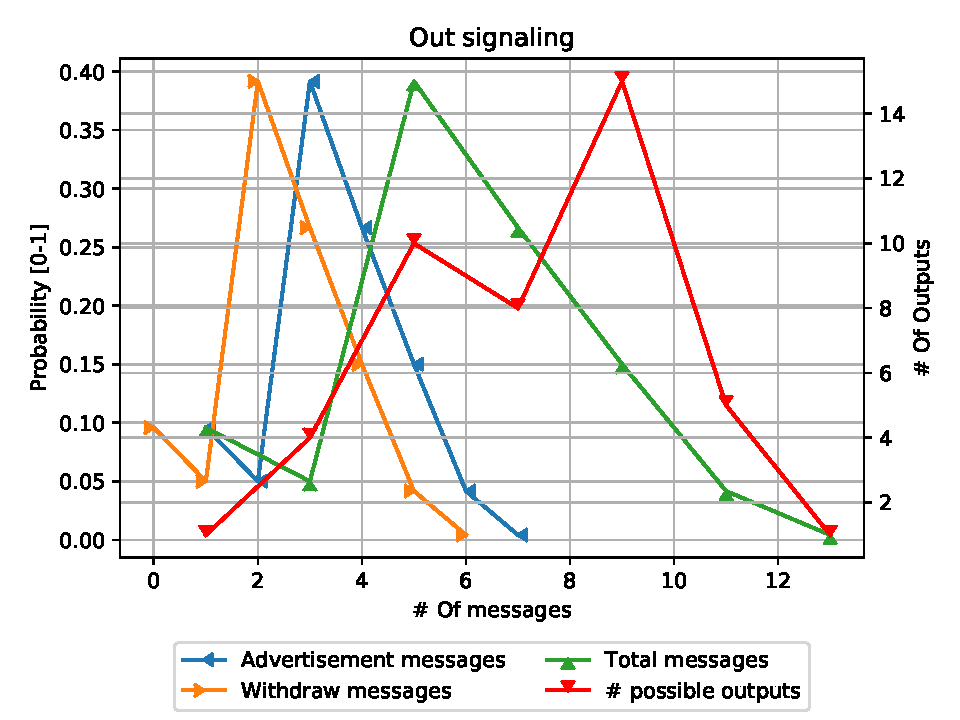
\includegraphics[width=\textwidth]{images/signal_study/fabrikant/30Fixed.pdf}
		 \caption{Node \num{8} output signals study with \textbf{\textit{Fixed \SI{30}{\second}}} strategy}
         \label{fig:signal_node9_fabrikant_fixed30_noIW}
     \end{subfigure}
     \hfill
     \begin{subfigure}[b]{0.49\textwidth}
         \centering
         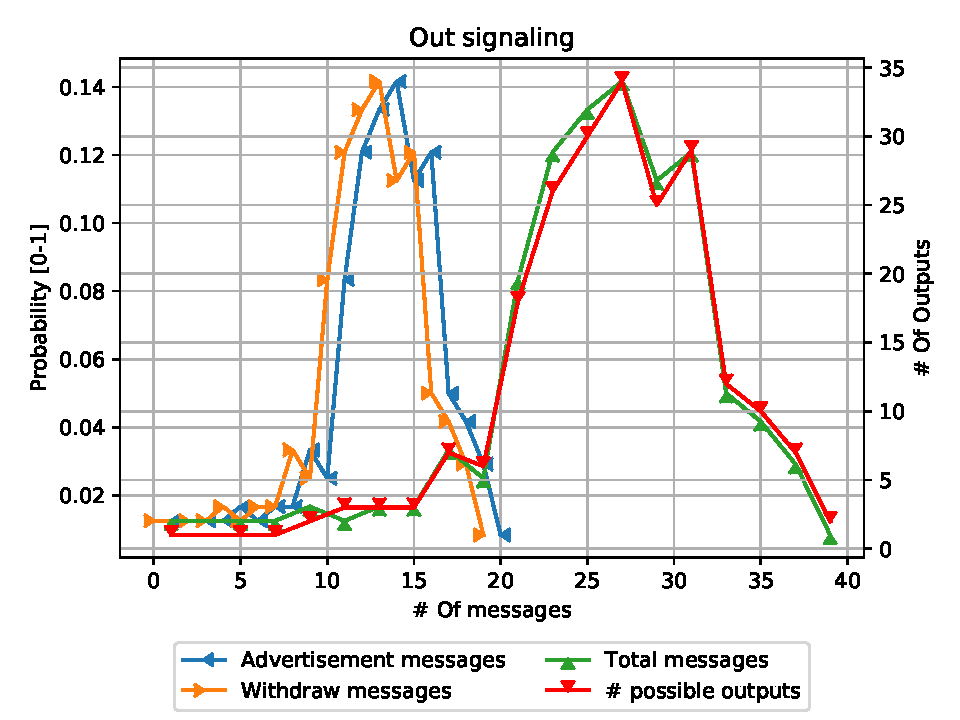
\includegraphics[width=\textwidth]{images/signal_study/fabrikant/Descendent.pdf}
		 \caption{Node \num{9} output signals study with \textbf{\textit{Descendent}} strategy}
         \label{fig:signal_node9_fabrikant_descendent_noiw}
     \end{subfigure}
     \begin{subfigure}[b]{0.49\textwidth}
         \centering
         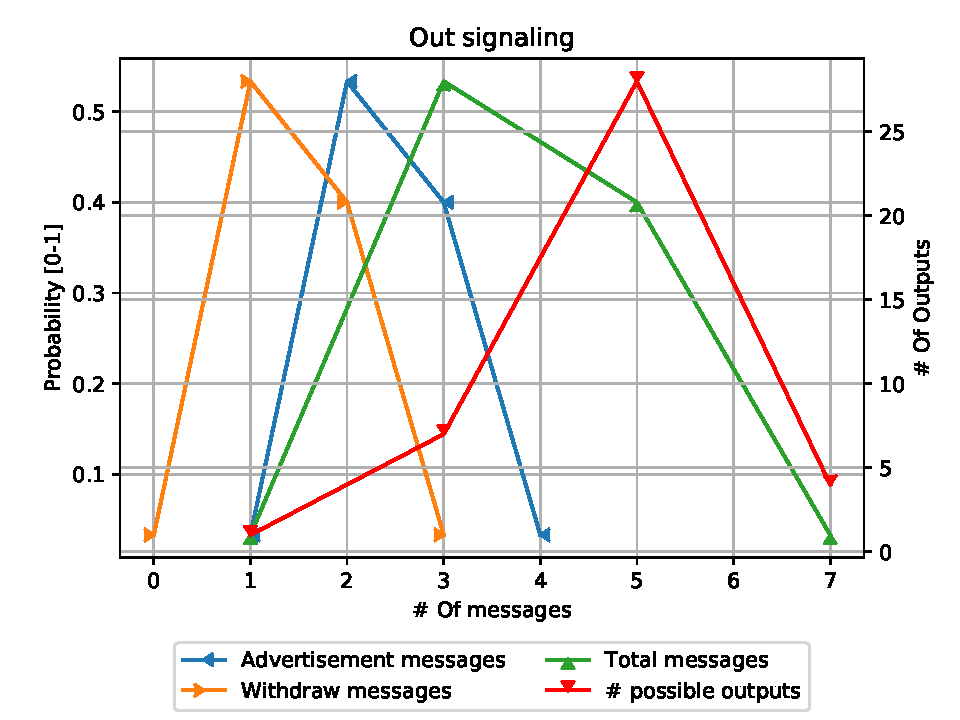
\includegraphics[width=\textwidth]{images/signal_study/fabrikant/Ascending.pdf}
		 \caption{Node \num{9} output signals study with \textbf{\textit{Ascendant}} strategy}
         \label{fig:signal_node9_fabrikant_ascendant_noIW}
     \end{subfigure}
		\caption{Output signal study of nodes \num{8} of the graph
			\Cref{fig:fabrikant_topology} with an input signal of \q{AWA} from node $d$
			with the \textbf{\textit{Fixed \SI{30}{\second}}}, \textbf{\textit{Descendent}}
			and \textbf{\textit{Ascendant}}	strategies, without the help of the \ac{IW}}
        \label{fig:signal_fabrikant}
\end{figure}

For simplicity I decided to study only the output signals caused by the sequence
\q{AWA} and without considering the \textit{No MRAI} case, results presented in
\Cref{fig:signal_fabrikant}.
The first signal study, \Cref{fig:signal_node9_fabrikant_fixed30_noIW}, is the
one that represents the actual standard value of the protocol~\cite{rfc4271}.
We can notice in that particular output study that the maximum detected length of
a signal is \num{13} and it's the last likely output, while the most probable
output length is \num{5}.
While, we can infer the \textit{Path Exploration} problem by the spike of unique
output signals with a length of \num{9}, this represent that the node experienced multiple
changes in its decisions.
The worst-case scenario is the one represented by \cref{fig:signal_node9_fabrikant_descendent_noiw}
where the maximum length of the output signal reaches almost \num{40} messages, but
the most probable output signal has a length between \num{20} and \num{30}.
This is the marker of a lot of decision changes in the best path for the destination.
Opposite to that case, we found the \textit{Ascendant} strategy in
\Cref{fig:signal_node9_fabrikant_ascendant_noIW} where the output
signals never used more than \num{7} messages.
In this last scenario we don't see a clear appearance of the \textit{Path Exploration}
problem, due to the fact that the node \num{8} is the last of the chain and
the \ac{MRAI} values permits to the other nodes to shares almost their best
possible path.

In conclusion of this chapter, we can say without doubts that \ac{MRAI} influences
the performances, confirming what has been presented in~\cite{fabrikant2011there},
that an incorrect setting of it can lead to an explosion in terms of messages.
And by consequence, to an explosion on the number of states and transitions.
Making difficult infer the initial sequence knowing only the output signal.
It is also noticeable that a different set of \ac{MRAI} values can also lead
to a better scenario than the standard one.
An alternative to the standard \ac{MRAI} has been already presented in~\cite{milani2020improving}
with the use of centrality metrics.
Is possible to study, other than specific nodes in the network also the performances
of all the sets of \ac{BGP} speaker, in order to study the impact of \ac{MRAI}
in general and what can affect it.
